\chapter{Approach}
\label{sec:approach}
\IMRADlabel{methods}
% \todo{State that generated schedules are checked by LLVM for correctness}

In the remainder of this chapter, we present the approach used for this thesis (compare~\Cref{fig:approach:overview}).
We start with explaining the necessary modifications to the build steps in \Cref{sec:approach:build_process}.
Then we discuss the importance of basic blocks for instruction scheduling in general and our approach specifically~(\Cref{sec:approach:basicblock}).
In \Cref{sec:approach:feasibility-study}, we present a feasability study to validate the potential of our approach.
That is followed by explaining the \ac{mcts} approach~(\Cref{subsec:approach:ml:mcts}), which is used to find well performing instruction schedules.
We introduce our approach to train inference models~(\Cref{subsec:approach:ml:global}) from the many \ac{mcts} models.
Finally, we discuss how we transform source code into data in a format that we can use for our data-driven approaches in \Cref{sec:approach:data-generation}.
\begin{figure}
    \centering
    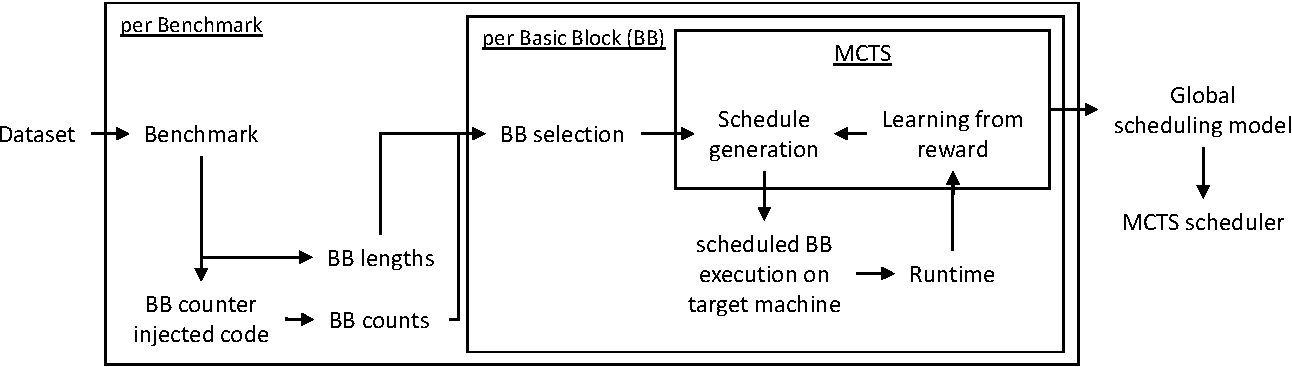
\includegraphics[width=\textwidth]{img/ppt/approach_overview-crop.pdf}
    \caption[Overview Over the Approach]{Overview over the complete approach:
    First, we evaluate the basic blocks in the programs of the LLVM Test Suite (\Cref{sec:bg:test-suite}) with our heuristics, described in \Cref{sec:approach:basicblock}.
    Then, we extract the selected basic blocks and normalize them for isolated execution (\Cref{sec:approach:bbisolation}).
    We train a \ac{mcts} model for each basic block (\Cref{subsec:approach:ml:mcts}), which includes measuring the runtime (\Cref{sec:approach:datageneration:runtime_methods}).
    Finally, we use the \ac{mcts} models to train various inference models (\Cref{subsec:approach:ml:global}).
    }
    \label{fig:approach:overview}
\end{figure}

\section{Build Process}
\label{sec:approach:build_process}
This section describes the process that we use for building the programs in the LLVM Test Suite (see \Cref{sec:bg:test-suite}).
First, we divide the compilation into separate steps to gain full controll over the settings.
We explain this in \Cref{sec:approach:divided-build}.
Next, \Cref{sec:approach:llvm-passes} explains the LLVM passes that we implement to add functionality to the LLVM compiler.

\subsection{Divided Process}
\label{sec:approach:divided-build}
The test suite comes with Makefiles and CMake configurations to automatically build all benchmarks.
However, these are not sufficient for our approach.
We need a modified build process for all the benchmarks because we are manipulating it in several cases.
Furthermore, the compilation cannot be done by a single command because not all arguments of the separate compilation steps are available in the compilers front-end.
We execute the front-end, optimization, and back-end compiler phases separately to have complete control over the build process.

We, further, analyze the CMake configurations of the programs in the LLVM test suite and extract required compiler arguments on a per benchmark level.
We categorize the extracted arguments into front-end, optimizer, and back-end phases.
Finally, we append them to the previously described arguments in the respective compilation phase.

Some programs read data from files or require arguments when calling them.
We analyze the test suite for these execution arguments.
To execute the test suite programs, we generate a shell script that calls the compiled benchmark with the required arguments.

\subsubsection{Front-End}
We have to set some compiler arguments to make the LLVM compiler front-end output LLVM \ac{ir} instead of compiling the program to an executable format.
We use the compiler front-ends \lstinline{clang}~\footnote{\url{https://clang.llvm.org/}} for C programs and \lstinline{clang++}\footnotemark[1] for C++ programs, both in version 12.0.0.
The compiler arguments are the same for both front-ends.
We pass the following arguments to the front-ends:
\begin{itemize}
    \item \lstinline{-O0}: To prevent optimization in this first step.
    \item \lstinline{-Xclang -disable-O0-optnone}: The \lstinline{-O0} flag alone also prevents optimization in later compilation stages. These flags still allow later optimizations.
    \item \lstinline{-S -emit-llvm}: To emit LLVM \ac{ir} for further processing --- instead of creating the program's binary.
\end{itemize}

\subsubsection{Optimizer}
The LLVM optimizer \lstinline{opt}~\footnote{\url{https://llvm.org/docs/CommandGuide/opt.html}} gives a choice to select one of the predefined optimization levels or select specific optimizer runs.
When we compile a benchmark for measuring the runtime, we only use the flag \lstinline{-O3} for optimizing the LLVM \ac{ir}.
This optimizes the code only on the \ac{ir} level, and does not interfere with the instruction scheduling.
We choose to use optimization in this step because it would usually be used in a production setting, too.
This makes the input code to our instruction scheduler more realistic to real-world situations.

We implement various LLVM passes that we explain in detail in \Cref{sec:approach:llvm-passes}.
The optimizer argument \mbox{\iloc{-passes=\emph{<pass-names>}}} activates these passes.

\subsubsection{Back-End}
The LLVM back-end compiler implements one instruction scheduling phase before the register allocation and one after the register allocation.
The first instruction scheduling phase is the one that we are interested in.
This first instruction scheduling phase was re-implemented in the LLVM project in the last years.
Both versions do currently work.
We decide to base our work on the old implementation because, the most target architectures still use it.

We manipulate the back-end by passing arguments to the LLVM static compiler \lstinline{llc}~\footnote{\url{https://llvm.org/docs/CommandGuide/llc.html}}.
This program represents the back-end phase and executes the instruction scheduling.
We use the following arguments for the back-end:
\begin{itemize}
    \item \lstinline{--pre-RA-sched=}: To select our new instruction schedulers for the pre-register-allocation phase.
    \item \lstinline{--misched-cutoff=0}: To disable the new pre-register-allocation scheduler implementation.
    \item \lstinline{--disable-post-ra}: To disable the post-register-allocation scheduler, because we focus on optimizing the pre-register-allocation phase and do not want the post-register-allocation scheduler to manipulate our schedules. Thereby, we create a controlled environment.
\end{itemize}

\subsection{LLVM Compiler Passes}
\label{sec:approach:llvm-passes}
The LLVM compiler framework makes it easy to implement compiler passes, which are functions that are executed during compilation and can modify the \ac{ir} code.
We implemented three of these functions: to count the number of executions of basic blocks, to count the basic block lengths, and to measure the runtime of a given function.
To make these passes usable, we compile them together with the source code of the LLVM compiler framework.

\subsubsection{Basic Block Execution Counting Pass}
\label{sec:approach:pass-count}
We implement an LLVM optimizer pass for injecting counters into a program that count the number of executions for each basic block.
Optimizer passes take LLVM \ac{ir} files as input and output the code in the same file format.
Our pass injects one global 64-bit counter variable for each basic block into the code.
Next, the pass adds instructions into the beginning of each basic block, which increases the corresponding counter by one.
At the end of the main function, the pass adds a format string and injects a call to the \lstinline{printf} function to print all the counter values and corresponding basic block names.

We include the optimizer pass into our build process (see \Cref{sec:approach:build_process}).
To actually get the execution counts, we build a program with this optimizer pass and execute it.
The benchmark then prints the counter values.

\subsubsection{Basic Block Instruction Count Pass}
\label{sec:approach:instr-count}
In order to get the number of instructions for all the basic blocks in a program we implement another pass.
This pass just prints the name of the basic block and its number of instructions to the command line during compile time.
It is a pure analysis pass and does not modify the \ac{ir} code.

\subsubsection{Function Runtime Measure Pass}
Lastly, we implement a pass, to measure the runtime of a single function.
The pass searches for the function that contains the selected basic block.
Then, it injects calls to the timer functions of the C++ standard library (\lstinline|std::high_resolution_clock::now|).
The calls are injected at the beginning of the given function and right before the return statement.
Additionally, it injects a compilation-unit-wide global variable and stores the measurements into this variable.
In the destructor of that compilation-unit, the pass injects code to print all the measurements.

\subsection{Instruction Scheduler Integration}
Since the LLVM compiler framework is designed to be easily extendable, it is not complicated to implement new instruction schedulers in C++.
However, these instruction schedulers must be compiled with the whole framework.
Additionally, due to C++'s complexity, it is not the best language for making quick experiments.

Therefore, we implement an LLVM instruction scheduler in C++ that calls an external command for scheduling selected basic blocks and and fallsback to another instruction scheduler for other basic blocks.
We define an interface to exchange scheduling information and write the information about the \ac{dag}'s structure and instructions to a text file.
Then our C++ scheduler calls an external shell command.
The executed command is responsible to generate another text file with the scheduled basic block.
Our C++ scheduler then parses the schedule and and schedules it.
We rely on LLVM's internal methods to ensure that the generated schedules are legal.
Our actual instruction schedulers that, \eg interact with the \ac{mcts} model are implemented in Python.

\section{Basic Block Selection Heuristics}
\label{sec:approach:basicblock}
Even though there is research on instruction scheduling on more extensive units (see \Cref{sec:rw:instruction-scheduling}), most compilers schedule instructions on a per basic block level.
This is also true for the LLVM compiler framework.
The advantage of this is that the limited scope avoids complicated situations and thus simplifies the scheduling problem.
For example, we do not have to deal with unclear execution paths due to conditional jump instructions.

Consequently, we also choose the basic block as the unit for instruction scheduling.
That means that we execute our experiments on individual basic blocks and thus, learn to schedule individual basic blocks.
Later, we combine the \ac{mcts} models to generalize the knowledge with our inference models to apply them to unseen basic blocks.
We describe this process in detail in \Cref{sec:approach:ml}.

Not all basic blocks provide an equal value to our experiments.
It also consumes too much time to work on all the basic blocks within the scope of this thesis (\eg compilation time, execution time, machine learning training time).
Therefore, we sort our basic blocks by heuristics. 
From this list, we select as many as we need and can handle in our experiments.
We design three heuristics which we explain in the following paragraphs.
See \Cref{tab:approach:bb_heuristics} for an example basic block with these heuristics.

\begin{table}
    \centering
    \begin{tabular}{@{}llrrr@{}}
        \toprule
        Function & Basic Block & Length & \(\#\) Executions & Product \\
        \midrule
        kernel\_floyd\_warshall\_StrictFP & for.body6 & 23 & 536,870,912 & 12,348,030,976 \\
        kernel\_floyd\_warshall & for.body6 & 23 & 536,870,912 & 12,348,030,976 \\
        print\_element & entry & 25 & 1,048,576 & 26,214,400 \\
        kernel\_floyd\_warshall\_StrictFP & for.cond4.preheader & 17 & 1,048,576 & 17,825,792 \\
        \(\cdots\) & \(\cdots\) & \(\cdots\) & \(\cdots\) & \(\cdots\) \\
        xmalloc & entry & 8 & 2 & 16 \\
        main & entry & 11 & 1 & 11 \\
        \bottomrule
    \end{tabular}
    \caption[Basic Block Heuristics for the Floyd-Warshall Benchmark]
    {
        The tables shows an excerpt of the basic block heuristics (see \Cref{sec:approach:basicblock}) for the floyd-warshall benchmark. 
        The basic blocks are sorted by the last heuristic, which is the product of the length and execution count. 
        From this list the table shows the top four and last two basic blocks in the benchmark.
    }
    \label{tab:approach:bb_heuristics}
\end{table}

\subsection{Longest Basic Blocks}
There are multiple reasons why we are more interested in longer basic blocks than in shorter basic blocks.
All these reasons summarize to the fact that there are more optimization possibilities with longer basic blocks.
We better exploit pipeline effects with longer basic blocks, because more instructions can potentially be executed interleaved (see \Cref{sec:bg:cpu}). 
With more instructions, there is potentially also a higher variety of instructions, which means that we can utilize more execution units on the processor in parallel.
Lastly, with short basic blocks, we only make few scheduling decisions per basic block. 
Summarized, this means that optimizations have a bigger effect on long basic blocks than on short basic blocks.
This was also shown by \citeauthor{stefanovic1997character}~\cite{stefanovic1997character}.

We use the optimizer pass described in \Cref{sec:approach:instr-count} to count the number of instructions per basic block.
From the output of that pass, we put together a list with all basic blocks and their lengths (see \Cref{tab:approach:bb_heuristics}).

\subsection{Most Executed Basic Blocks}
Some basic blocks are significantly more often executed than others.
For example, basic blocks in the bodies of loops run often.
A basic block in the error checking code in the beginning of a program might only execute once.
Often executed basic blocks influence the overall runtime a lot.
Hence, we are more interested in optimizing these.
We count the number of executions with the LLVM optimizer pass described in \Cref{sec:approach:pass-count}.


\subsection{Most Executed and Longest Basic Blocks}
\label{sec:approach:basicblock:exec-long}
The previous two heuristics are helpful on their own, but we are most interested in basic blocks that combine the two aspects.
For example, the most executed basic block can still come from a very simple loop with few instructions in the loop body.
We compute the product of the two heuristics to get a combined heuristic.

\section{Feasibility Study}
\label{sec:approach:feasibility-study}
Before starting to optimize a process, it is useful to determine whether there is potential for any optimizations.
Therefore, we show, that different instruction schedules can indeed lead to different runtimes on our target hardware (see \Cref{sec:eval:hw}).
This early experiment is also helpful to get an overview of how much the runtime can vary between different instruction schedules.

% select longest bb per benchmark
% longest might have the most possible schedule, so more variation in the random schedules
\Cref{sec:bg:test-suite} describes the selection of benchmarks from the LLVM Test Suite.
For this experiment, we select one basic block per benchmark, whose instruction schedule we modify.
For the selection of basic blocks we use the heuristic that balances between the most executions and the longest basic blocks, which is discussed in \Cref{sec:approach:basicblock:exec-long}.

% measure the function runtime
% we measure the runtime of the function (implemented llvm passes)
% talk about impact on measurements.
We execute this experiment in an early stage and did not have a basic block extraction pipeline nor means to measure the execution time of a single basic block.
Therefore, we execute the whole benchmark with the modified instruction schedule of a single basic block.
However, measuring the runtime of the whole benchmark includes the execution of much overhead code that we are not interested in.
Thus, we instead measure the runtime of the function that contains the basic block of interest.
This corresponds to the third method in \Cref{fig:approach:runtime_scopes}.

% generate 10 different random schedules 
% do that twice
The simplest approach to achieve this experiments goal is to use random instruction schedules.
Our random instruction scheduler works on top of a basic list scheduler.
This means, out of the issue-ready instructions provided by the list scheduler, our scheduler chooses one at random.
This is repeated until no more instructions are left.
We fix the seed of the random number generator for reproducibility and generate instruction schedules with the seeds 0-10 for each selected basic block.
The basic block of interest might execute multiple times in the measured function for reasons discussed in \Cref{sec:approach:runtime-measurement-unit}.
We choose the shortest measured runtime per benchmark run to ensure that we use the same execution path in our measurements.
To check that the runtime measurements are reproducible, we run each generated instruction schedule two times.

% evaluate
To carry out this experiment, we choose a processor with the architecture AArch64 and the \auroralong{}.
The choice is explained in \Cref{sec:eval:hw}.
\Cref{fig:eval:rndm:aarch64} shows a representative selection of experimental results for the AArch64 processor.
\begin{figure}
    \begin{subfigure}{0.0325\textwidth}\caption{}\label{fig:eval:rndm:aarch64:a}\end{subfigure}
    \begin{subfigure}{0.44\textwidth}
        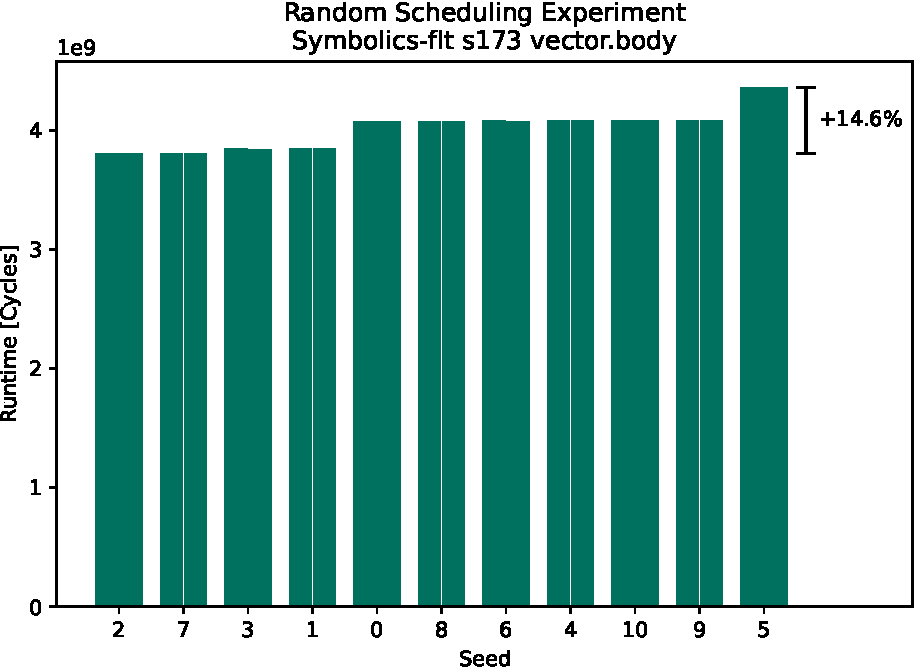
\includegraphics[width=\textwidth]{img/random-scheduling-experiment-pi-collected/Symbolics-flt-crop.pdf}
    \end{subfigure}
    \hfill
    \begin{subfigure}{0.0325\textwidth}\caption{}\label{fig:eval:rndm:aarch64:b}\end{subfigure}
    \begin{subfigure}{0.44\textwidth}
        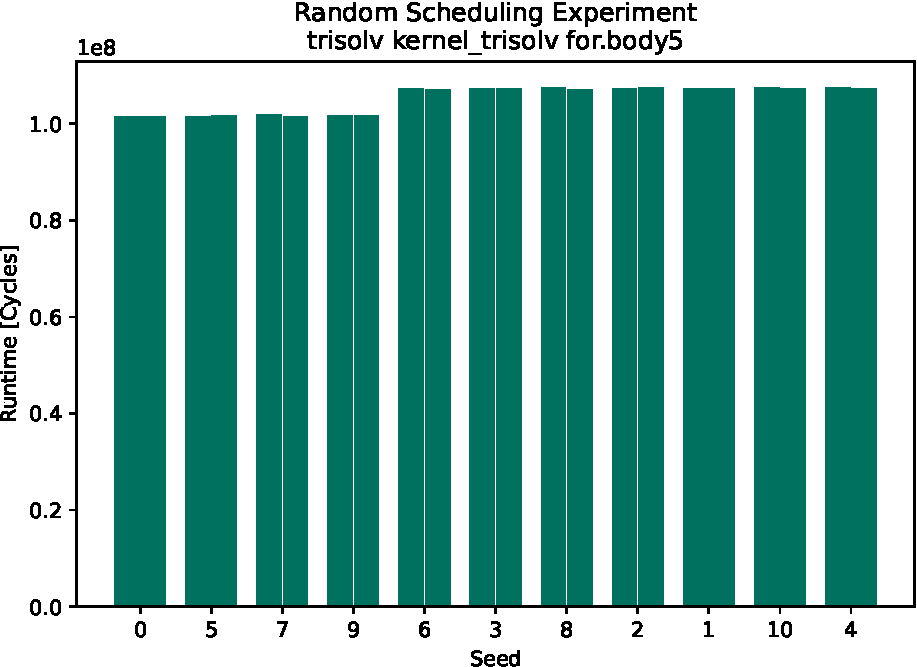
\includegraphics[width=\textwidth]{img/random-scheduling-experiment-pi-collected/trisolv-crop.pdf}
    \end{subfigure}

    \vspace{0.5cm}
    \begin{subfigure}{0.0325\textwidth}\caption{}\label{fig:eval:rndm:aarch64:c}\end{subfigure}
    \begin{subfigure}{0.44\textwidth}
        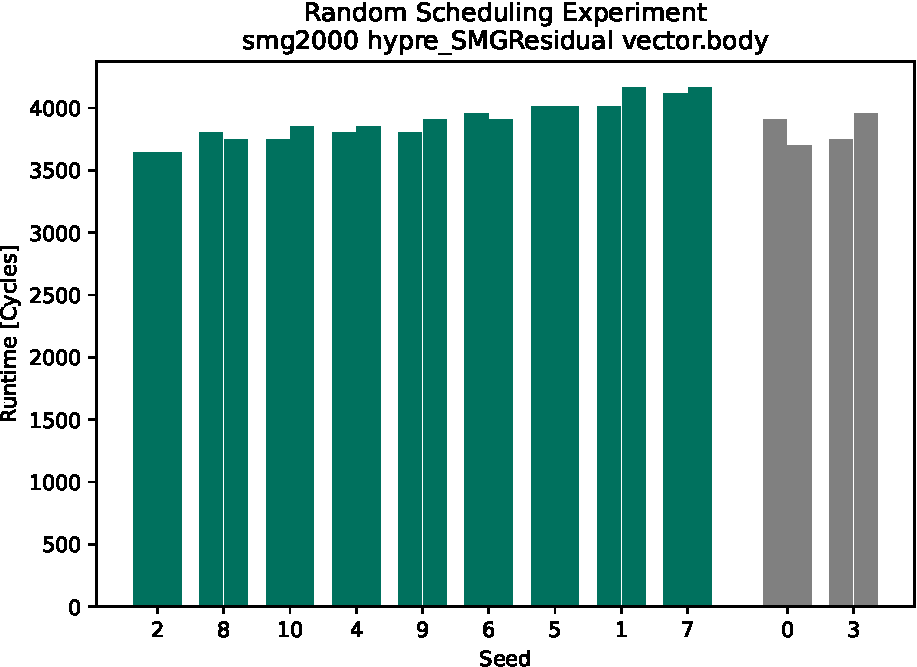
\includegraphics[width=\textwidth]{img/random-scheduling-experiment-pi-collected/smg2000-crop.pdf}
    \end{subfigure}
    \hfill
    \begin{subfigure}{0.0325\textwidth}\caption{}\label{fig:eval:rndm:aarch64:d}\end{subfigure}
    \begin{subfigure}{0.44\textwidth}
        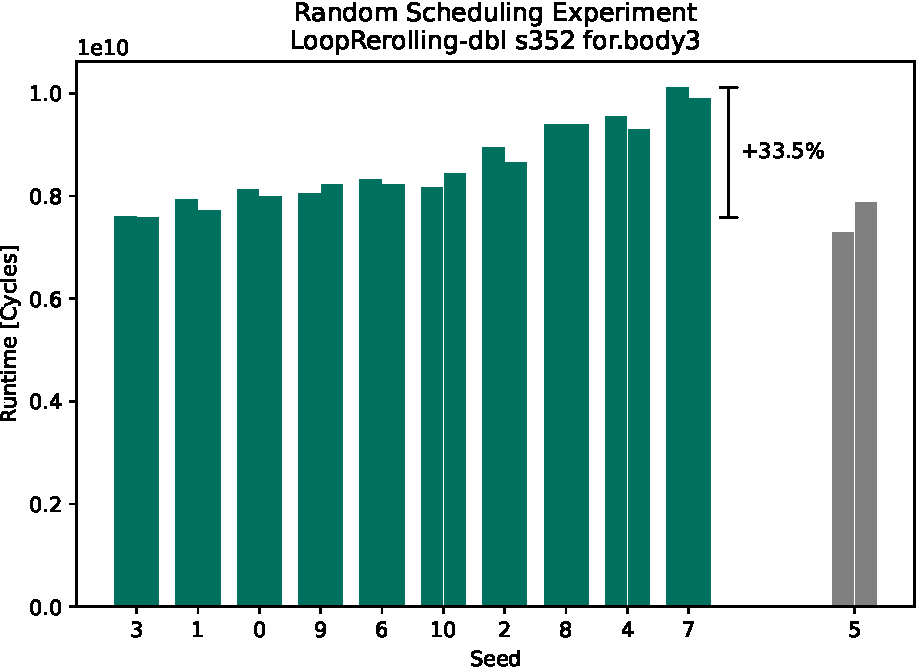
\includegraphics[width=\textwidth]{img/random-scheduling-experiment-pi-collected/LoopRerolling-dbl-crop.pdf}
    \end{subfigure}

    \vspace{0.5cm}
    \begin{subfigure}{0.0325\textwidth}\caption{}\label{fig:eval:rndm:aarch64:e}\end{subfigure}
    \begin{subfigure}{0.44\textwidth}
        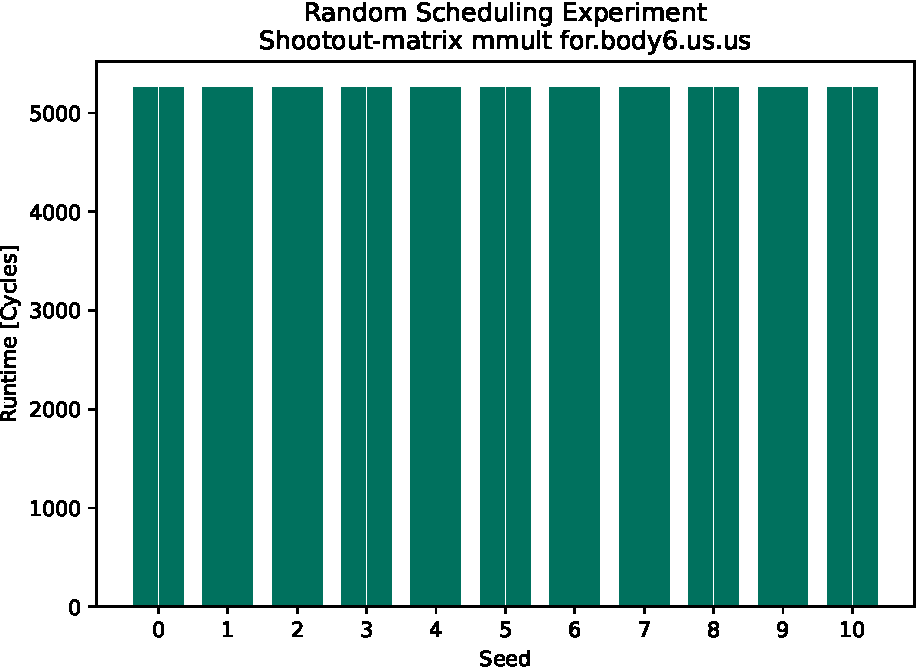
\includegraphics[width=\textwidth]{img/random-scheduling-experiment-pi-collected/Shootout-matrix-crop.pdf}
    \end{subfigure}
    \hfill
    \begin{subfigure}{0.0325\textwidth}\caption{}\label{fig:eval:rndm:aarch64:f}\end{subfigure}
    \begin{subfigure}{0.44\textwidth}
        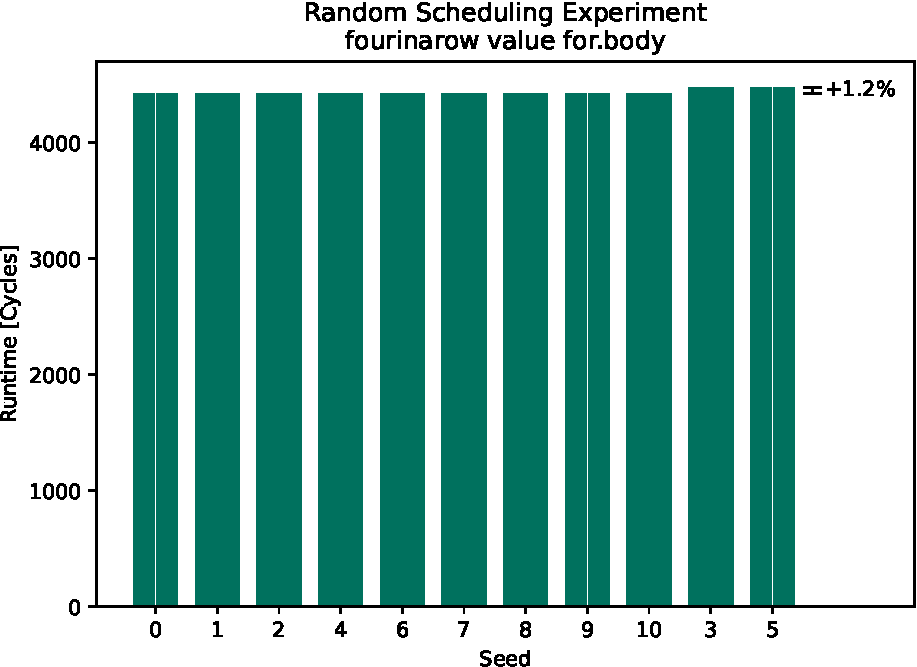
\includegraphics[width=\textwidth]{img/random-scheduling-experiment-pi-collected/fourinarow-crop.pdf}
    \end{subfigure}

    \caption[Random Scheduling Experiment on AArch64]{Random Scheduling Experiment on AArch64:
    The bars show the runtime of a function with a random instruction schedule.
    The two runs of the instruction schedule are grouped together.
    The distance measure represents the longest execution time relative to the shortest execution time.
    Two runs that differ more than 5\% are marked as outliers and plotted in gray.}
    \label{fig:eval:rndm:aarch64}
\end{figure}
The plots show the runtimes grouped by the different seeds for the random instruction scheduler.
Runtimes that differ between two runs more than 5\% are marked as outliers and plotted in gray.
\Crefrange*{fig:eval:rndm:aarch64:a}{fig:eval:rndm:aarch64:d} show examples where different runtimes are clearly observable for different instruction schedules.
However, this is not always observable.
\Cref{fig:eval:rndm:aarch64:e} and \Cref{fig:eval:rndm:aarch64:f} show examples where no difference in the runtime was observable.
% The average coeffecient of variation over the basic blocks is 0.035.
In summary, we see that different instruction schedules can generate measurable differences in the runtime.
This means that there is potential for improvements.

\Cref{fig:eval:rndm:aurora} shows a similar selection for the same experiment on the \aurora{} processor.
\begin{figure}
    \begin{subfigure}{0.0325\textwidth}\caption{}\label{fig:eval:rndm:aurora:a}\end{subfigure}
    \begin{subfigure}{0.44\textwidth}
        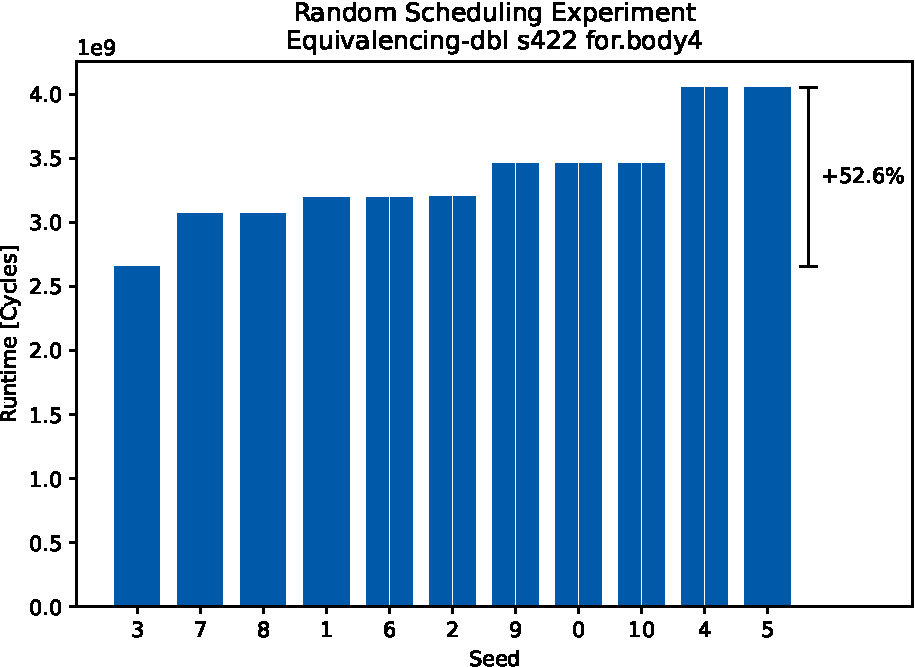
\includegraphics[width=\textwidth]{img/random-scheduling-experiment-aurora-collected/Equivalencing-dbl-crop.pdf}
    \end{subfigure}
    \hfill
    \begin{subfigure}{0.0325\textwidth}\caption{}\label{fig:eval:rndm:aurora:b}\end{subfigure}
    \begin{subfigure}{0.44\textwidth}
        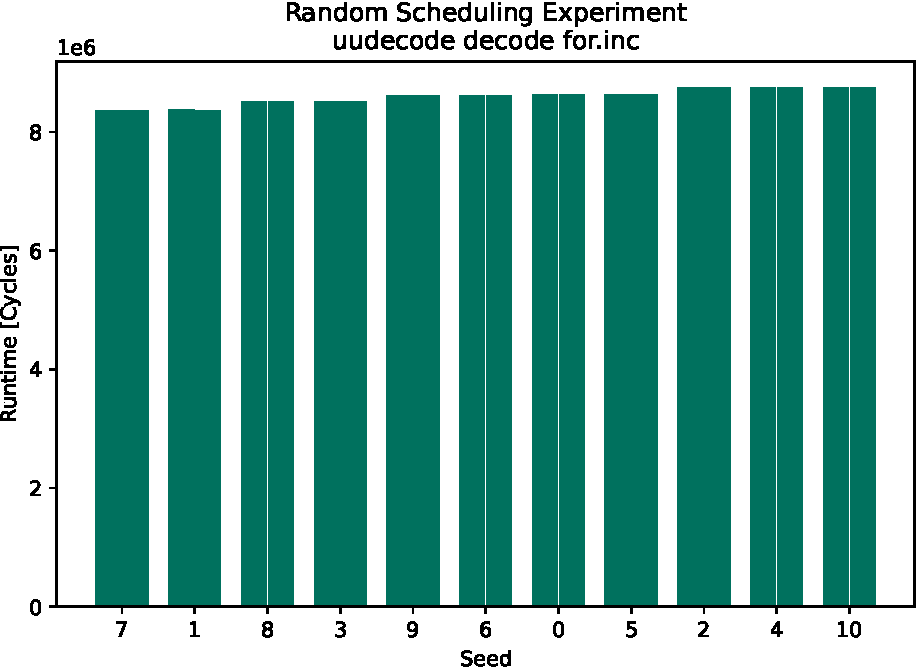
\includegraphics[width=\textwidth]{img/random-scheduling-experiment-aurora-collected/uudecode-crop.pdf}
    \end{subfigure}

    \vspace{0.5cm}
    \begin{subfigure}{0.0325\textwidth}\caption{}\label{fig:eval:rndm:aurora:c}\end{subfigure}
    \begin{subfigure}{0.44\textwidth}
        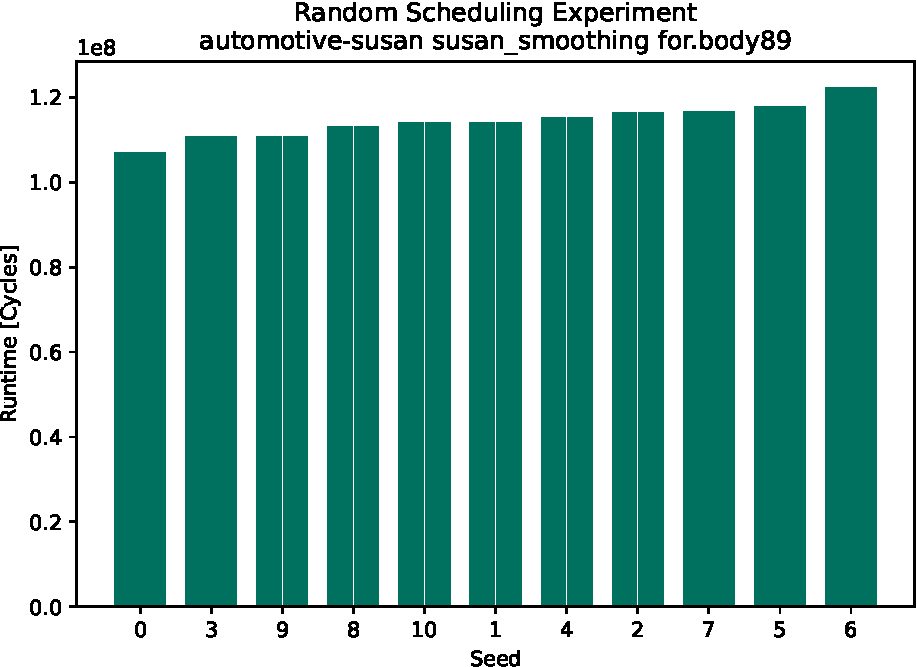
\includegraphics[width=\textwidth]{img/random-scheduling-experiment-aurora-collected/automotive-susan-crop.pdf}
    \end{subfigure}
    \hfill
    \begin{subfigure}{0.0325\textwidth}\caption{}\label{fig:eval:rndm:aurora:d}\end{subfigure}
    \begin{subfigure}{0.44\textwidth}
        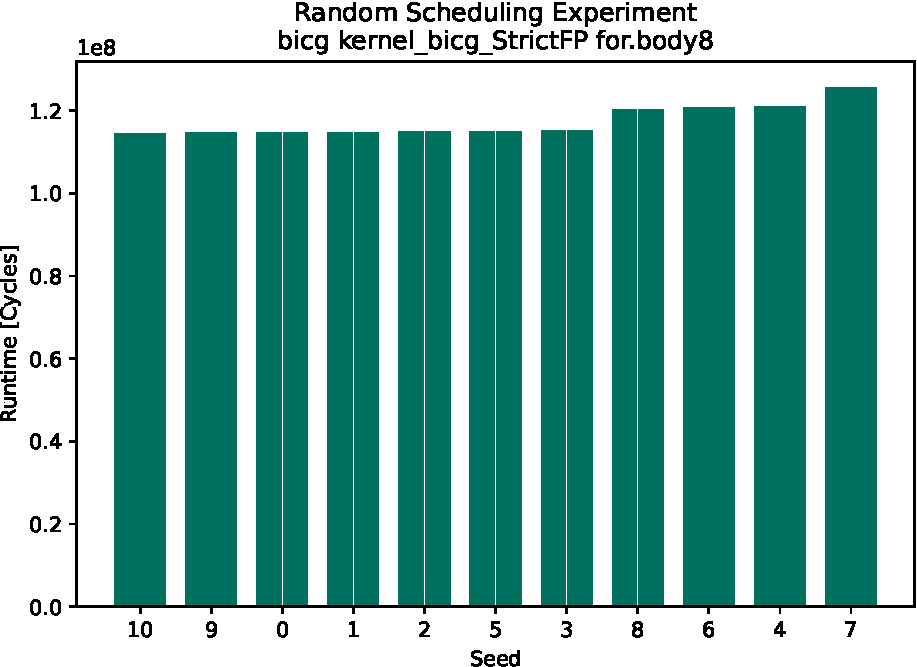
\includegraphics[width=\textwidth]{img/random-scheduling-experiment-aurora-collected/bicg-crop.pdf}
    \end{subfigure}

    \vspace{0.5cm}
    \begin{subfigure}{0.0325\textwidth}\caption{}\label{fig:eval:rndm:aurora:e}\end{subfigure}
    \begin{subfigure}{0.44\textwidth}
        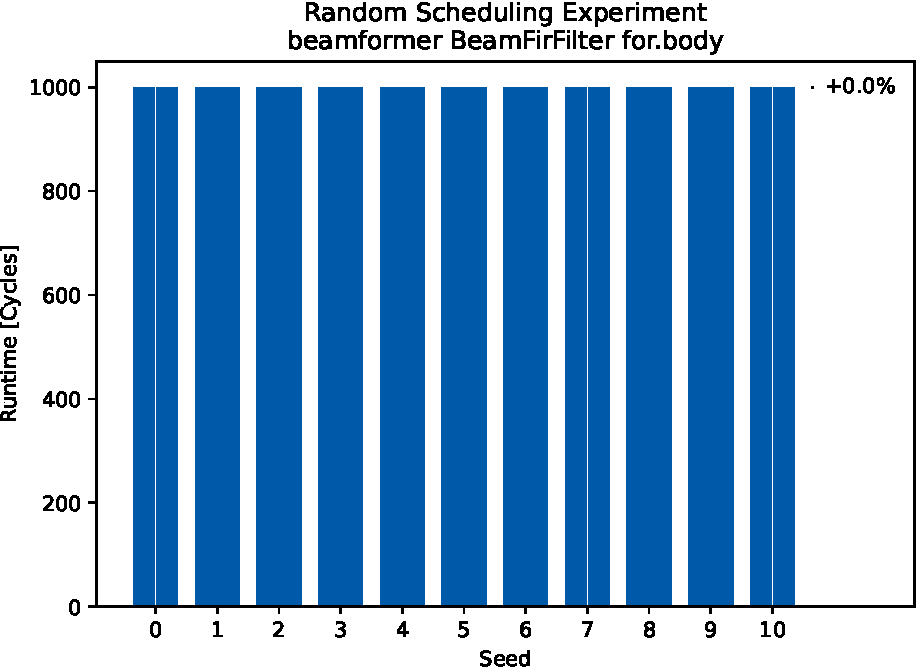
\includegraphics[width=\textwidth]{img/random-scheduling-experiment-aurora-collected/beamformer-crop.pdf}
    \end{subfigure}
    \hfill
    \begin{subfigure}{0.0325\textwidth}\caption{}\label{fig:eval:rndm:aurora:f}\end{subfigure}
    \begin{subfigure}{0.44\textwidth}
        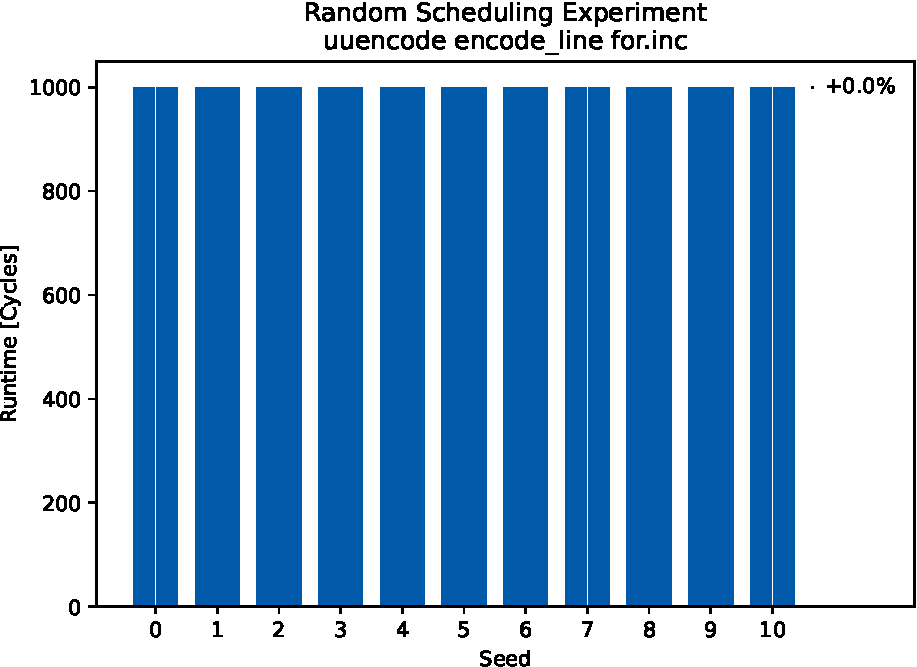
\includegraphics[width=\textwidth]{img/random-scheduling-experiment-aurora-collected/uuencode-crop.pdf}
    \end{subfigure}

    \caption[Random Scheduling Experiment on \auroralong{}]{Random Scheduling Experiment on \auroralong{}:
    The bars show the runtime of a function with a random instruction schedule.
    The two runs of the instruction schedule are grouped together.
    The distance measure represents the longest execution time relative to the shortest execution time.
    Two runs that differ more than 5\% are marked as outliers.
    However, this processor did not produce any outliers in our experiment.}
    \label{fig:eval:rndm:aurora}
\end{figure}
We can observe a similar outcome of the experiment.
However, as this processor cannot be interrupted by the \ac{os}, the runtimes are more stable between two runs.
In fact, no measurements in the whole example where marked as outliers.
% The average coeffecient of variation over the basic blocks is 0.046.
In summary, we observe potential for optimizations on this processor, as well.

Multiple reasons could lead to the small or missing variations that we observe in \Crefrange{fig:eval:rndm:aarch64:e}{fig:eval:rndm:aarch64:f} and \Crefrange{fig:eval:rndm:aurora:e}{fig:eval:rndm:aurora:f}:
One possibility is that different instruction schedules have no effect on the runtime of the basic block.
The motivation for this experiment was to verify, that these cases do not dominate the instruction schedules.
Other possibilities have their origin in the experimental setup, these could be:
\begin{itemize}
    \item The basic block for which we manipulate the instruction schedule might have a low influence on the runtime of the function.
        We tried to minimize this effect by choosing basic blocks that are often executed.
    \item Our random instruction scheduler works on top of LLVM.
        In this stage of the back-end, LLVM makes still use of pseudo-instructions that are not represented in the binary.
        This means that schedules that we see as different schedules might actually end up being equal in the binary.
    \item There are short functions with a short execution time.
        We observed few changes in the runtime when the measured execution time is below 1,000 processor cycles.
        The underlying timer of the C++ standard library might not be able to measure such short time periods.  
\end{itemize}
However, the experiment is still valid, because we show that we are able to influence the runtime by manipulating the instruction schedules beyond noise in the measurements.

In summary, we observe different runtimes for different instruction schedules and the results are reproducible over multiple runs.
This is not true for all basic blocks, but the goal of this experiment was to show the existence of an effect of the instruction schedule on the runtime.
These results motivate further research with two goals:
First, to automatically optimizing instruction scheduling for basic blocks.
Secondly, to do that only for basic blocks that influence the runtime a lot in order to speed up compilation times.

\section{Learning to Schedule}
\label{sec:approach:ml}
Our goal is to create a model that can generate good instruction schedules for basic blocks.
Therefore, we have to define a mapping that we want to learn with this model.
The possible inputs can be complex, like characteristics of the hardware, the register states, or others.
However, we decided for this thesis to begin with a simple model and limit our input to the $n$ last scheduled instructions and the set of instructions that can be scheduled.
These are important because they might utilize different execution units on the processor, and thus generate pipeline effects.

We define this mapping as
\begin{equation}
    (h_n, \ldots, h_1) \times \{i_1, \ldots, i_m\} \mapsto i_k
    \label{eqn:mlmapping1}
\end{equation}
where $h$ defines the instructions in the history of scheduled instructions, $i$ are candidate instructions that are ready to be scheduled and $k \in \{1, \ldots, m\}$.
However, we define a second, easier to implement, mapping
\begin{equation}
    (h_n, \ldots, h_1) \times i \mapsto r
    \label{eqn:mlmapping2}
\end{equation}
where we map from the history and a single instruction to a reward value $r$.
We lose some input information in this model about the other candidate instructions.
But we can now simply run the model for all the available instructions and select the one with the best reward.

We need lots of data samples to utilize data-driven, or machine learning approaches.
One way would be to generate valid random schedules.
The downside of this approach is that we generate many bad schedules because the better ones are rare.
A better way is to use \ac{mcts} to iteratively find better schedules (see \Cref{subsec:approach:ml:mcts}).
The \ac{mcts} approach searches for good schedules locally, \ie for a single basic block.
So, the search is not generalized for other basic blocks.

There are two reasons why we add a second step to our approach:
First, the \ac{mcts} approach takes a lot of time to complete and is not usable for production environments.
Second, this approach only works locally on single basic blocks.
To generate a model that works globally, \ie also for unseen basic blocks, we add a second step and learn from the locally good schedules.
Therefore, we extract data samples matching the input format of \Cref{eqn:mlmapping1}, or respectively \Cref{eqn:mlmapping2}.
We have trained different models that are explained in detail in \Cref{subsec:approach:ml:global}.

\subsection{Monte Carlo Tree Search for Instruction Schedules}
\label{subsec:approach:ml:mcts}
We choose \ac{mcts} to find instruction schedules that perform best for a given basic block.
The reason is that this approach fits naturally for sequential problems and allows us to balance between the exploration and exploitation of instruction schedules. 
\ac{mcts} tries all possible next steps in a given situation and chooses the further steps randomly because there is no information available.
When all possibilities in a situation are already examined, the algorithm takes the best option (based on a defined metric) and tries to improve from thereon.
It does not choose the best option every time but also incorporates exploration choices.
This enables us to search for good instruction schedules.
See \Cref{sec:bg:mcts} for more details.

% Explain structure of the tree: nodes = instructions, edges = valid traversion of dag
The input to our \ac{mcts} approach is a \ac{dag} generated by the LLVM compiler, which defines the valid instruction schedules.
See \Cref{fig:bg:llvm-dag} for an example.
The LLVM instruction \ac{dag} still contains many instructions that exist just for internal reasons and are not translated to machine instructions.
We remove these pseudo-instructions from the instruction \ac{dag} and adjust the dependencies between the nodes.

The nodes in an \ac{mcts} tree represent a state in the underlying model, and the edges correspond to transitions between these states.
Compare \Cref{fig:approach:max-vs-avg} to see that our \ac{mcts} nodes represent a partial instruction schedule.
The edges in our \ac{mcts} tree represent a legal scheduling of a new instruction to the previous schedule.
When we iterate back from any node to the root node, we get the partial instruction schedule in reverse ordering.
\begin{figure}[p]
    \centering
    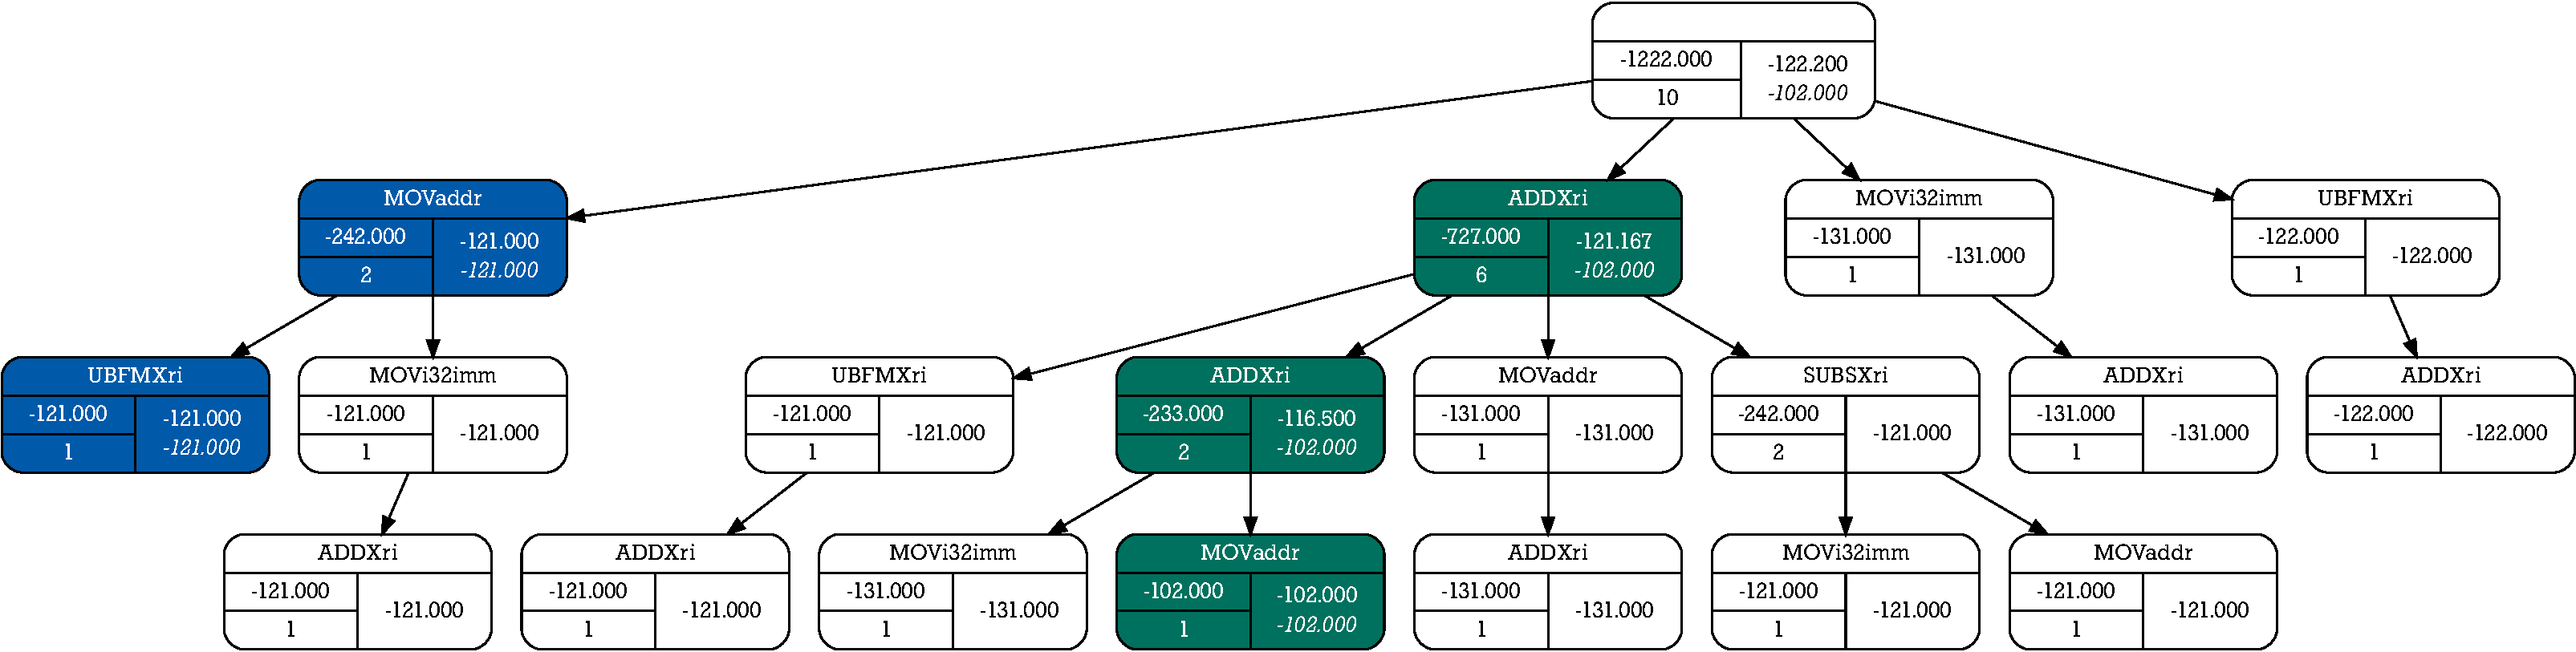
\includegraphics[width=18cm,angle=90]{data/mcts-max-vs-avg/svg/selected/8752639012199.inkscape-crop.pdf}
    \caption[\ac{mcts} Tree with the Consequences of Maximum and Average Metric]{
        \ac{mcts} tree with the consequences of maximum and average metric:
        The boxes represent a \ac{mcts} node, at the top is the name of the instruction, on the left are the cumuluated metric and the number of visits, on the right is the metric.
        The colored nodes have two metric values: The upper one is the average metric value and the lower italic one shows the maximum metric value.
        In this example, we use the negative runtime for the metric.
        The blue nodes show the path that was selected when we used the \ac{mcts} approach with the average metric.
        There is a path of green nodes which shows the path that would have been selected if we used the maximum metric.
        The green path results in a better metric value.
        % \\ (Benchmark: LoopRestructuring-dbl, Function: s2233, Basic Block: for.body20)
    }
    \label{fig:approach:max-vs-avg}
\end{figure}

We do not use the default choice of node evaluation metric.
Typically, to evaluate the reward of a node in the \ac{mcts} tree, the algorithm compute the average of the child nodes.
In our approach, this leads to situations where we have already found a good schedule but keep searching for schedules in another area of the tree.
The reason for that is that the good schedule might be surrounded by relatively bad schedules, which have a negative effect on the average evaluation.
When we train \ac{mcts} for games, that makes sense because we do not want to get into situations where only one good state exists, and the surrounding ones would let us lose the game.
But we are only interested in a single best schedule, therefore we do not care about similar but bad schedules.
Thus, we do not take the average but the maximum.
This means that in the exploitation phase, we always follow the path to the best-found schedule.
\Cref{fig:approach:max-vs-avg} illustrates the effects of both metrics, where the green path represents the maximum metric and the blue path represents the average metric.
Our approach is similar to the one in~\cite{bjornsson2009cadiaplayer}.
However, they still use the average for the search part, which we do not.

% Explain process: Generate schedule -> compile -> measure runtime -> train mcts -> go to 1
The \ac{mcts} learning process is separated into four phases:
\begin{enumerate}
    \item Generate schedule: \\
    Apply the exploration or exploitation selection phase and generate a new schedule based on the previous experience.
    This results in the most situations in a partial instruction schedule because the \ac{mcts} tree usually not grows until it knows all states.
    The partial instruction schedules are completed by using random scheduling decisions. 
    \item Compile the generated schedule: \\
    The generated schedule is transformed into a C++ file with a function that contains the inline assembly of the scheduled basic block.
    We then compile the schedule with our benchmarking framework (see \Cref{sec:approach:isol_bb_exec}).
    \item Execute and measure the runtime: \\
    The compiled executable is transferred to our target machine and executed there to measure the runtime of the basic block (see \Cref{sec:approach:isol_bb_exec}).
    \item Progress the \ac{mcts} tree with the measured runtime: \\
    Then, the measurement data is copied back to the machine where we run the \ac{mcts} training.
    The measurement data is preprocessed and used to train the \ac{mcts} tree.
\end{enumerate}
This process is repeated many times, depending on the experiment.
See \Cref{sec:bg:mcts} for more information.

% Technically possible to use for production, but slow
Note that this \ac{mcts} approach is not only able to generate data for our global model.
It can theoretically also be used in a normal compilation process.
It is not practical to use it for a whole program because of the extra compilation steps, caused by the many experiments.
However, critical parts of a program could be optimized with this approach.

% Positive sideeffect: Also there to define a possible range of improvement
A positive side effect of this \ac{mcts} approach is that we generate an upper limit for the improvements of the instruction scheduling phase.
The further we grow the \ac{mcts} tree, the higher is the probability that we find the actual upper limit of improvements.
This is at the same time an upper limit for the global inference models in our second step.
Therefore, we can see how much of our potential improvements we are able to reach with our inference models.

\subsection{Inference Models}
\label{subsec:approach:ml:global}
Once we have found good schedules by generating \ac{mcts} trees for many basic blocks, we want to generalize this knowledge for unknown basic blocks.
This is necessary to transfer the knowledge to unseen basic blocks and make the model usable in practice by generating good schedules directly, in contrast to searching them with \ac{mcts}.
Therefore, we have developed three different models that we discuss here.

Another way to see this two-step approach is to see the \ac{mcts} step as a training phase and this global model step as inference phase, thus the name.

\subsubsection{Nearest Neighbor Model}
\label{sec:app:nearest-neighbor}
Our first model is a nearest neighbor approach.
That means we iterate our \ac{mcts} trees and build up a big look-up model in which we can search for situations and see what decision performed best.

% Dataformat: (h_n, ..., h_1) x (i_1, i_2) -> (w_1, d, w_2)
In order to build the model, we first define the input and output formats.
A scheduling situation has the format
\begin{equation}
    (h_n, \ldots, h_1) \times {i_1, \ldots, i_m}
    \label{eqn:approach:example-scheduling-situation}
\end{equation}
where instructions $h$ build a sequence of last scheduled instructions and instructions $i$ build the set of candidate instructions.
To simplify our model and have more data per scheduling situation, we limited the size of the set of candidate instructions to two.
The disadvantage is that we lose context information on other candidates.
The data we are interested in per scheduling situation is the number of times instruction $x$ was better than instruction $y$ or vice versa and the number of times they were on par.
This results in the data format
\begin{equation}
    (h_n, \ldots, h_1) \times (i_1, i_2) \mapsto (w_1, d, w_2)
\end{equation}
where $w_1$ and $w_2$ represent how often instruction $i_1$, or $i_2$ was the better choice.
How often they were on par is counted by the variable $d$.

% How to build this model?
To build the model, we iterate the \ac{mcts} trees and extract the contained data.
\begin{figure}
    \centering
    \begin{forest}
        [$h_n$
            [$\vdots$
                [$h_1$
                    [$i_1$] [$i_2 $] [$i_3$]
                ]
            ]
        ]
    \end{forest}
    \caption[Example Scheduling Situation]{Example scheduling situation with the previously scheduled instructions $h$ and the candidate instructions $i$ to choose from.}
    \label{fig:approach:example-scheduling-situation}
\end{figure}
For every scheduling situation (compare \Cref{eqn:approach:example-scheduling-situation}), we take every combination of instructions $i$.
In the example in \Cref{fig:approach:example-scheduling-situation}, that would be $(i_1, i_2)$, $(i_1, i_3)$, and $(i_2, i_3)$.
For each combination, we check which instruction choice resulted in a better reward.
We add this situation to our model if it was not already present.
Otherwise, we increase the corresponding counter variable in this situation.

In addition to this situation, we can also learn from this situation for a scheduling situation with a shorter history.
So we also add the situation for all partial histories.
For example, when we have a scheduling situation with the history $(h_3, h_2, h_1)$, we also add our learnings to the model with the histories $(h_2, h_1)$, $(h_1)$, and the empty history $()$.

% How to make scheduling decisions from this model?
This model can be easily applied for scheduling.
In a given scheduling situation, we just search for the history and all combinations of available instructions.
If we have found all the combinations, we can make our decision based on the counts.
For the situation where we did not find all the required combinations, we define a percentage threshold $t_c$.
If we found more than $t_c$ instruction combinations, we make a choice based on the instructions that we have found.
If we found fewer than $t_c$ instructions, we remove the oldest instruction $h_n$ from the history and search again for all the instruction combinations. 

\subsubsection{Support Vector Machine Model}
% What mapping are we trying to learn?
Further, we want to learn parametric regression models.
Therefore, we use a different mapping that we learn because the inputs and outputs are scalar values.
\begin{equation}
    (h_n, \ldots, h_1) \times i \times (d_{min}, d_{max}) \mapsto r
    \label{eqn:approach:regression-mapping}
\end{equation}
We choose to have a sequence of history instructions $(h_n, \ldots, h_1)$ with a defined length $n$.
From the history and the candidate instruction $i$ we map to the reward value extracted from the \ac{mcts} data.

One additional metric that we add to our input is the distance into the history of the direct \ac{dag} predecessor instructions.
We do this because, instructions have to wait for the result of the direct predecessor instructions when they have a data dependency.
And the bigger the distance between them is, the higher is the probability, that the predecessors already terminated. 
For example, instruction $a$ depends on instruction $b$, and we are in the situation in which we want to schedule $a$.
That means we have already scheduled $b$.
There are usually also other instructions that we scheduled after $b$.
We count the number of instructions that we scheduled between $a$ and $b$.
There is typically more than one instruction that $a$ depends on, so we decided to take the maximum and the minimum number of instructions between $a$ and its predecessors for the dataset.
We refer to these values as $d_{max}$ and $d_{min}$ in \Cref{eqn:approach:regression-mapping}.

% How was the input data generated?
To build a dataset with the mapping defined in \Cref{eqn:approach:regression-mapping} we iterate the \ac{mcts} trees.
For every instruction node, we collect its previously scheduled instructions and its reward value.

% Data preprocessing
However, we cannot insert these data points into the \ac{svm} model because it requires numerical values only.
We transform the instructions from their textual representation into an ordinal encoding, \ie every instruction gets a unique numerical representation.
Further, we scale all numerical values into the range $[0,1]$ because \acp{svm} typically learn better when inputs are in this range.

With this data, we train an \ac{svm} regression model.
The details and results of the experiments can be found in \Cref{sec:eval:svm}.

\subsubsection{Neural Network Model}
We choose to use a neural network as a second regression model, because they have a shorter inference runtime than \acp{svm} when trained on big datasets.
With this model, we try to learn the same mapping as we did with our \ac{svr} model, which is defined in \Cref{eqn:approach:regression-mapping}.
Consequently, we use the same dataset that we have already built for the \ac{svr} model.

In contrast to our \ac{svr} model, we chose not to encode the instructions into ordinary values.
The instructions are encoded into one-hot vectors because neural networks can handle high-dimensional inputs better.
Further, we also scale numerical values into the range $[0,1]$, like we did for the \ac{svr} model.

We use a standard neural network with three hidden layers with dimensions 512, 128, and 64.
The output layer is a singular value which represents the scaled score of the given scheduling situation.
All hidden layers are followed by a ReLU activation function~\cite{nair2010rectified}.
We use the Adam optimizer~\cite{kingma2014adam} with a learning rate of $10^{-3}$.
For the loss function, we use the squared error.
We discuss the details and results in \Cref{sec:eval:nn}.

\section{Data Generation}
\label{sec:approach:data-generation}
We cannot build our data-driven models (see \Cref{sec:approach:ml}) directly from the programs in the LLVM Test Suite (\Cref{sec:bg:test-suite}), as it requires some transformation from the code to a metric.
Many metrics can be chosen for optimization, \eg runtime, energy consumption, cache misses, processor stalls.
We focus on optimizing the instruction scheduling for short runtimes.
To generate data for our MCTS approach, we need a mapping from instruction schedules to runtimes.

The most reliable approach is to measure the runtime while executing the code.
However, research on approaches that rely on analytical models exists, see \Cref{sec:rw:other:runtime} %~\cite{llvm:mca, mendis2019ithemal, taha2003instruction, laukemann2018automated}.
We choose the classical approach of runtime measurements since we have access to the hardware, and the resulting data will be more accurate.
Therefore, we compile the code with varying instruction schedules and execute it to measure its runtime.
We discuss various aspects of this in the remainder of this section.

\begin{figure}
    \centering
    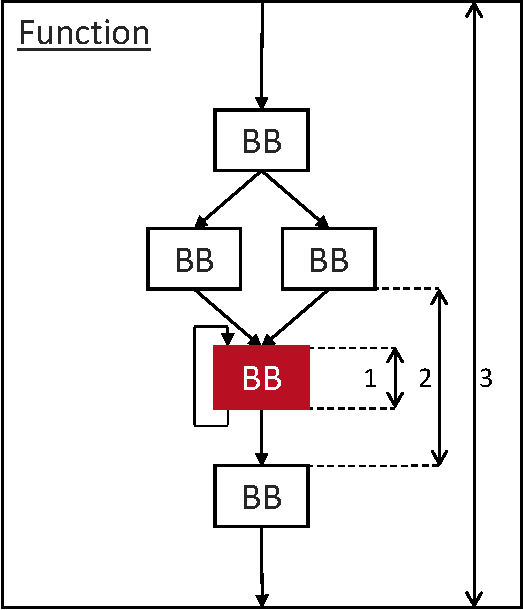
\includegraphics[scale=0.8]{img/ppt/runtime_measurement_scopes-crop.pdf}
    \caption[Possibile Scopes for Measuring Runtimes]{The outer box represents a function. 
    The function consists of multiple basic blocks (BB) where different possible branches are caused by if/else statements and loops. 
    The diagram shows three possible runtime measuring scopes to measure the runtime of the filled basic block.
    Method 1 shows a measuring inside of a basic block. 
    With method 2, the measurement starts with the end of the last basic block and ends with the start of the next one.
    Method 3 measures the complete function which surrounds the basic block.}
    \label{fig:approach:runtime_scopes}
\end{figure}

\subsection{Runtime Measurement Unit}
\label{sec:approach:runtime-measurement-unit}
The metric we are interested in specifically is the relative runtime compared to a baseline runtime.
Runtime overheads can be ignored, as long as they are constant over multiple runs and the baseline has the same overheads.
Thus, there are various possibilities for placing the start and stop events of the timer to accomplish runtime measurements of fractions of the application's code.
The objective is to minimize noise and get reliable, reproducible measurements.
We discuss the possibilities of making measurements on a basic block, function, and application scope and relevant aspects to these possibilities.

\subsubsection{Application}
\label{sec:approach:datageneration:runtime:app}
The most straightforward approach to measuring the runtime of a piece of code is to measure the runtime of its whole application.
The disadvantage is that we include many more instructions in the measurement than we are interested in.
This generates lots of noise from various possible sources (\eg from \ac{io} instructions like opening files, printing to the screen, or varying latencies for memory accesses).
Also, the longer the runtime of a program, the higher is the probability that the operating system interrupts the execution for more important processes.
Depending on the used measurement method (see \Cref{sec:approach:datageneration:runtime_methods}), this may be included or not be included in the measurement.
These disadvantages make this approach unreliable and not usable for us because we are interested in the short runtime of a single basic block.

\subsubsection{Function}
\label{sec:approach:datageneration:runtime:function}
A finer-grained approach is to start the timer at the beginning of the function or method that contains the basic block of interest and stop the timer at the end of the function (see Method 3 in \Cref{fig:approach:runtime_scopes}).
This approach creates several problems.

Compared to measuring the runtime of the whole application, this approach executes only a small fraction of the code.
This results in a lower degree of variance in the measured runtimes due to fewer \ac{os} interruptions, and fewer memory and \ac{io} accesses.
Thus, the precision of these measurements is higher.

Note in \Cref{fig:approach:runtime_scopes}, that different control paths are possible in a function, based on if/else statements or loops.
This can be problematic in a general setup.
However, the benchmarks we use and the data we insert to them are deterministic, \ie the same paths are taken in each benchmark execution.
Theoretically, if there was no variance in the measurements, the shortest measured execution time will always correspond to the same execution path.
In practice, we get many varying measurements because of different execution paths.
That makes it difficult to differentiate between execution paths and variance in the measurements.

\subsubsection{Basic Block}
The most intuitive approach when scheduling basic blocks is to measure only the runtime of the basic block we are interested in.
We eliminate all extra instructions that we are not interested in.
However, we can still get runtime variations for different reasons:
\begin{itemize}
    \item The basic block could call other functions which could, in turn, execute varying branches. 
          See \Cref{sec:approach:bbisolation} for a discussion about this.
    \item The \ac{os} could interrupt the execution. 
          But the probability decreases with shorter code fragments.
\end{itemize}

One requirement that can not be met in all situations is that of a very precise timer.
These timers usually depend on the hardware directly, \ie the hardware must provide such functionality to measure runtimes.
This is possible on our chosen hardware and is discussed in more detail in \Cref{sec:approach:hwpercounter}.

Thus, as this is a feasible solution for our experiments, we have chosen to measure the runtime of basic blocks alone.
    
\subsection{Runtime Measurement Methods}
\label{sec:approach:datageneration:runtime_methods}
% \todo{Could add little experiment where we compare hardware timers vs OS access}
Various possibilities to observe execution times exist in systems that we use for our research.
These can typically be classified into the categories of profiling, \ac{os} utilities, or hardware utilities.
We discuss these three in more detail.

\subsubsection{Profiling}
Profilers (\eg gperf \cite{graham1982gprof}) are programs that observe the execution of other processes running on the system.
They are designed to observe the execution from start to end and to return various metrics. 
Some examples are execution times per function, memory consumption, and cache misses.
The observation is done by taking snapshots of the process of interest.
Thus, profilers are good for finding, \eg performance problems and memory leaks in software.

However, we need cycle-accurate measurements from instruction A to instruction B for our experiments.
Profilers are not able to make such precise measurements, \ie they are not helpful to us because they are designed for other purposes.

\subsubsection{Operating System Methods}
\acp{os} typically need to work with time values and also provide a programming interface to use its timing functions.
There is the wall clock time and timers that are based on \ac{cpu} functionality to get times.
We are interested in the latter.
Often there are various possibilities to retrieve timing values from the hardware with varying precision.
The most precise timers are usually good for measuring intervals in the microseconds range or longer.
\ac{os} functions have some overhead because they also handle various errors.
\begin{table}
    \centering
    \begin{tabular}{@{}ll@{}}
        \toprule
        Operating System & Timer in C language \\
        \midrule
        Linux & \lstinline|clock_gettime()| \\
        Windows & \lstinline|QueryPerformanceCounter()| \\
        \bottomrule
    \end{tabular}
    \caption[Operating System Interfaces to Their Timing Functions]
    {
        The table shows examples for interfaces in \acp{os} to their timing functions in the C programming language.
    }
    \label{tab:approach:timing_functions}
\end{table}
See \Cref{tab:approach:timing_functions} for selected \acp{os}.
The C++ function \lstinline|std::high_resolution_clock()| from the standard library falls back to one of these \ac{os} functions.

Some \acp{os} not only provide timing methods, but also allow to manage how a process executes.
Linux provides different methods to avoid or reduce the probability of \ac{os} interrupts during the execution of a process.
\begin{itemize}
    \item Isolating \ac{cpu} cores: 
    The Linux kernel command line option \mbox{\iloc{isolcpus=\emph{<cpu-number>}}} in the boot loader instructs Linux to not schedule tasks to the given \ac{cpu} cores automatically.
    \item Pinning a process to a \ac{cpu} core: 
    The Linux program \lstinline|taskset| configures the \ac{os} to schedule processes to specific \ac{cpu} cores.
    This can also be used to schedule processes on isolated \ac{cpu} cores.
\end{itemize}
If we pin a process to an isolated \ac{cpu} core, this task will not be interrupted by the \ac{os}.
This makes the measuring of runtimes more reliable.

\subsubsection{Hardware Performance Counters}
\label{sec:approach:hwpercounter}
The most code blocks we want to measure are only 5-50 instructions long, \ie we need very precise measurements.
We use the assembly instructions of the given hardware directly to get the most precise timing values with the lowest overhead.
These instructions typically return the value of a processor cycle-counter.

Depending on the used high-level language and hardware, using assembly instructions can be complicated.
But it is not a problem in our experiments because the code blocks we want to measure are already written in the assembly language of the given hardware.
That means we only add a timer instruction at the beginning and one at the end.
We do some error checking after the execution has stopped (see \Cref{sec:approach:isol_bb_exec} for details).
\begin{table}
    \centering
    \begin{tabular}{@{}ll@{}}
        \toprule
        Hardware & Assembly instruction \\
        \midrule
        \auroralong{} & \lstinline|smir %s60, %usrcc| \\
        AArch64 & \lstinline|mrs x0, PMCCNTR_EL0| \\
        ARM32 & \lstinline|mrc p15m, 0, r0, c15, c12, 1| \\
        x86 & \lstinline|rdtsc| \\
        \bottomrule
    \end{tabular}
    \caption[Assembly Instructions for Getting the Cycle Counter Value of a Given Hardware]{Assembly instructions for getting the cycle counter value of a given hardware.}
    \label{tab:approach:asm_instrs_timing}
\end{table}
See \Cref{tab:approach:asm_instrs_timing} for the assembly instructions per hardware and \Cref{fig:approach:bb-executable} for an example.

Depending on the hardware and the \ac{os}, access to these instructions or registers might not be permitted.
For the AArch64 architecture and a Linux \ac{os}, we had to implement and load a kernel module that granted access to this register.
 
\subsection{Execution Unit}
\label{sec:approach:exec_unit}
Due to many iterations in the learning processes, we have to execute the differently scheduled basic blocks many times.
If we executed the whole benchmark that contains the basic block of interest, it would be time-intensive, and many lines of code were executed that we are not interested in.
This forces us to extract the basic block from the benchmark and execute it in isolation.
Here, we discuss the advantages and disadvantages of the two possible approaches.

\subsubsection{Benchmark}
The first option is to execute the complete benchmark for every new schedule that was generated during the learning process.
The advantage is that we execute the original basic block as it would appear in the real benchmark.
The problem with this approach is that the execution time of a benchmark can be high and makes the execution the bottleneck in our pipeline.
Many benchmarks in our dataset take several minutes to execute on a RaspberryPi 3B.
So, always executing the whole benchmark is costly to even get only one runtime measurement per schedule.
In order to get statistically relevant runtimes, we have to measure them multiple times.

\subsubsection{Basic Block}
The alternative to executing the whole benchmark is to extract the scheduled basic block from the benchmark and execute it in isolation.
By using this approach, we reduce the execution time to a minimum and do not execute code we are not interested in.
Consequently, we can execute the benchmark many times and get statistically reliable runtime measurements.
The disadvantage is that we have to slightly modify the basic block or the execution crashes.

\subsection{Basic Block Isolation}
\label{sec:approach:bbisolation}
As discussed in \Cref{sec:approach:exec_unit}, we are forced to execute basic blocks isolated from the benchmark.
To make a basic block executable, we isolate it, normalize it, and insert it as inline assembly into our minimal C++ framework.

\subsubsection{Basic Block Extraction}
First, we compile the benchmark and schedule the basic block with our modified compilation process (see \Cref{sec:approach:divided-build}) into assembly files.
Next, we extract the basic block instructions from the assembly file.
Then, we modify the basic block instructions to prevent execution and compilation errors, and as the last step, we inject it into our C++ framework.
We describe the modifications in the next paragraphs.

Assembly files contain comments, labels, and assembler directives which we remove.
Comments are useless lines for the execution task. 
The labels are not required, as we do not jump to other instructions.
Assembler directives represent commands to the assembler program for bookkeeping, storage reservation, and other purposes.
These could interfere with our compilation process and are also removed.

Basic blocks can contain jump instructions as the last instruction and function calls in any position.
We only schedule the instructions in the given basic block, so we are also only interested in its own runtime.
Executing other code, which could internally choose different paths, would add noise to our measurements.
To prevent this uncontrolled program execution, we simply remove jump and call instructions.
The removal of these instructions might slightly reduce the execution time, but the reduction is constant over all executions with different schedules.

In order to prevent segmentation faults, we have to redirect all memory accesses to a memory area that we are allowed to read and write to.
This affects all load and store instructions.
In our framework, we allocate 8 byte on the stack where we redirect all memory accesses.
This also means that all memory accesses are cache hits, and we have a controlled environment in this aspect.

\Cref{fig:approach:bb-cleaning} shows an example in which we manipulate a basic block.
We remove a label and comments, redirect memory accesses and remove a jump instruction.
\begin{figure}
    \begin{subfigure}{0.65\textwidth}
        \begin{lstlisting}
.LBB9_14:               // %for.body82
                        //   Parent Loop BB9_2 [..]
                        //     Parent Loop BB9_[..]
                        // =>    This Inner Loo[..]
sub	x24, x23, #8        // =8
cmn	x24, #8             // =8
ldr	d0, [x21]
ldr	d1, [x19, x23]
ldr	d2, [x22, #-8]!
ldr	d3, [x7, x23]
fmul	d2, d2, d3
fsub	d0, d0, d2
fdiv	d0, d0, d1
str	d0, [x21]
mov	x21, x22
mov	x23, x24
b.ne	.LBB9_14
        \end{lstlisting}
        \caption{Original assembly}
    \end{subfigure}
    \hfill
    \begin{subfigure}{0.3\textwidth}
        \begin{lstlisting}[showlines=true]




sub	x24, x23, #8
cmn	x24, #8
ldr	d0, [%2]
ldr	d1, [%2]
ldr	d2, [%2]
ldr	d3, [%2]
fmul	d2, d2, d3
fsub	d0, d0, d2
fdiv	d0, d0, d1
str	d0, [%2]
mov	x21, x22
mov	x23, x24

        \end{lstlisting}
        \caption{Manipulated assembly}
    \end{subfigure}
    \caption[Assembly Basic Block Manipulation]{AArch64 Assembly Basic Block Manipulation:
    We remove the first line because it is a label.
    We remove the comments in the lines two to 6.
    Then, we replace the memory accesses with the placeholder \lstinline|\%2|, which the compiler replaces later (see \Cref{fig:approach:bb-executable}).
    Lastly, we remove the jump instruction in line 17.}
    \label{fig:approach:bb-cleaning}
\end{figure}

\subsubsection{Isolated Basic Block Execution}
\label{sec:approach:isol_bb_exec}
To execute the extracted basic block, we have to surround it with some other code to generate a valid C/C++ program.
For this, we implement a small benchmarking framework.
\Cref{fig:approach:bb-executable} shows an example of the basic block from \Cref{fig:approach:bb-cleaning} integrated into this framework.
We also add the \ac{cpu} timer calls and mark the used registers as clobbered.
% This framework is compiled together with the given basic block in the inline assembly format.
The optimization is turned off in this compilation step, so the basic blocks are executed as given.
\begin{figure}
    \begin{lstlisting}[
        % language=C++
    ]
#pragma once

#include <cstdint>

struct Benchmark {
public:
    __attribute__((always_inline)) uint64_t operator() () {
        uint64_t a[4] = { 0xcdab, 0xcdab, 0xcdab, 0xcdab };
        uint64_t* p = a;
        uint64_t start, end;
        asm volatile(
            "mrs        %0, PMCCNTR_EL0 \n\t"
            "sub	x24, x23, #8	\n\t"
            "cmn	x24, #8         \n\t"
            "ldr	d0, [%2]	\n\t"
            "ldr	d1, [%2]	\n\t"
            "ldr	d2, [%2]	\n\t"
            "ldr	d3, [%2]	\n\t"
            "fmul	d2, d2, d3	\n\t"
            "fsub	d0, d0, d2	\n\t"
            "fdiv	d0, d0, d1	\n\t"
            "str	d0, [%2]	\n\t"
            "mov	x21, x22	\n\t"
            "mov	x23, x24	\n\t"
            "mrs        %1, PMCCNTR_EL0 \n\t"
            :  "=r"(start), "=r"(end)
            :  "r"(p)
            :  "q0", "q1", "q2", "q3", "x21", "x23", "x24",  "memory", "cc"
        );
        return end > start ? end - start : 0;
    }
};        
    \end{lstlisting}
    \caption[Assembly Basic Block Integration Into Execution Framework]{AArch64 Assembly Basic Block Integration into Execution Framework:
    This example shows the basic block from \Cref{fig:approach:bb-cleaning} how it is integrated into the C++ framework.
    The compiler replaces the placeholder \lstinline|\%2| with a pointer to the array \lstinline|a| (line 8).
    We also list the used registers, so the compiler knows that their values have changed (line 28).
    The first and the last instructions in the inline assembly (lines 12, 25) call the \ac{cpu} timer.}
    \label{fig:approach:bb-executable}
\end{figure}

The executable first executes the basic block in 100 warmup rounds to prevent side effects from caches and other reasons.
The actual execution where we measure the runtime is repeated until 1,000 valid measurements are done.
Invalid measurements can occur when the runtime is negative.
This happens when the cycle counter overflows.

\subsection{Computing Rewards From Runtimes}
Even though we do the warmup rounds, we still get few data points that are clearly outliers and should not be included in our experiments.
We sort the 1,000 runtime measurements and strip the top and bottom 50 measurements.
Spot checks have shown that we remove all the outliers in all the checked experiments.
\begin{table}
    \centering
    \begin{tabular}{@{}rr@{}}
        \toprule
        Runtime & Num. Occurances \\
        \midrule
        140 & 998 \\
        143 & 1 \\
        711 & 1 \\
        \bottomrule
    \end{tabular}
    \hspace{0.8cm}
    \begin{tabular}{@{}rr@{}}
        \toprule
        Runtime & Num. Occurances \\
        \midrule
        121 & 708 \\
        120 & 289 \\
        123 & 1 \\
        163 & 1 \\
        1491 & 1 \\
        \bottomrule
    \end{tabular}
    \hspace{0.8cm}
    \begin{tabular}{@{}rr@{}}
        \toprule
        Runtime & Num. Occurances \\
        \midrule
        114 & 994 \\
        121 & 2 \\
        115 & 1 \\
        129 & 1 \\
        130 & 1 \\
        694 & 1 \\
        \bottomrule
    \end{tabular}
    \caption[Example Runtime Measurement Distribution]{Example runtime measurement distribution for three different schedules.\\(Benchmark: almabench, Function: anpm, Basic Block: entry)}
    \label{tab:approach:example_runtimes}
\end{table}
See \Cref{tab:approach:example_runtimes} for an example with three different schedules for the same experiment.

Because different basic blocks have their different runtimes, the absolute measured speedups between two basic blocks are not comparable.
To have a metric $m$ that we can compare with all other basic blocks in the data set, we normalize the experiment runtime $r_e$ with the runtime of the baseline scheduler $r_b$.
\begin{equation}
    m=\frac{r_b}{r_e}
    \label{eqn:approach:mcts-score}
\end{equation}
